\slide{Plan}
{
% NOTE: each line starting with '% NOTE:' will be exported as a 'script.log', along with the section and file names.
% NOTE: this is a nice way of making a notes for you presentation.
% NOTE: ex. explain the plan in detail - forcus on point 4.
\tableofcontents
}


\section{Text}


\slide{Listing on multiple comulns}
{
% NOTE: talk alot here, as there is no point in doing anything usefull
% NOTE: do not sleep
% NOTE: remember to eat something
\begin{multicols}{2}
Lorem ipsum dolor sit amet, consectetur adipisicing elit, sed do eiusmod tempor incididunt ut labore et dolore magna aliqua. Ut enim ad minim veniam, quis nostrud exercitation ullamco laboris nisi ut aliquip ex ea commodo consequat. Duis aute irure dolor in reprehenderit in voluptate velit esse cillum dolore eu fugiat nulla pariatur. Excepteur sint occaecat cupidatat non proident, sunt in culpa qui officia deserunt mollit anim id est laborum.
\end{multicols}
}


\slide{Points}
{
\begin{itemize}
\item Item 1
\pause

\item Item 2
\begin{enumerate}
\item Enum 1
\item Enum 2
\end{enumerate}
\end{itemize}
}


\slide{Columns}
{
\begin{columns}

\begin{column}{0.45\textwidth}
\begin{itemize}
\item Alice
\item Has
\item A
\item Cat
\end{itemize}
\end{column}

\begin{column}{0.45\textwidth}
\begin{itemize}
\item Cat
\item Has
\item AIDS
\end{itemize}
\end{column}

\end{columns}
}


\slide{Message boxes}
{
\begin{block}{Famous quote}
Lorem ipsum dolor sit amet, consectetur adipisicing elit, sed do eiusmod tempor incididunt ut labore et dolore magna aliqua.
\end{block}
}


\slide{Font sizes}
{
\tiny{tiny} \\
\scriptsize{scriptsize} \\
\footnotesize{footnotesize} \\
\small{small} \\
\normalsize{normalsize} \\
\large{large} \\
\Large{Large} \\
\LARGE{LARGE} \\
\huge{huge} \\
\Huge{Huge}
}


\slide{Any questions so far?}
{
\begin{center}
\vspace{-10em}
\fontsize{160}{200}\selectfont ?
\end{center}
}


\section{Listings}


\slide{Test module}
{
\begin{itemize}
\item Modules end with "-m"
\item They are self-containing
\end{itemize}
\lstinputlisting{cpp/test-m.hpp}
}


\slide{Test function}
{
\begin{itemize}
\item Functions ends with "-f"
\item Content of file is wrapped into a function call
\end{itemize}
\lstinputlisting{cpp/other-f.hpp}
}


\slide{Multicolumn listing}
{
\tiny{}
\begin{multicols}{2}
\lstinputlisting{cpp/long_source-m.hpp}
\end{multicols}
}


\slide{Verbatim blocks}
{
\begin{itemize}
\item \emph{verbatim} does not work normally
\item \emph{fragile} does not work when inside \emph{newcommand}
\item \emph{semiverbatim} is prefferred
\item it may require some escaping though\ldots
\end{itemize}
\begin{semiverbatim}
some weird +!@\% text

it's fine \
\end{semiverbatim}
}


\section{Graphics}


\slide{Full-slide image}
{
\begin{center}
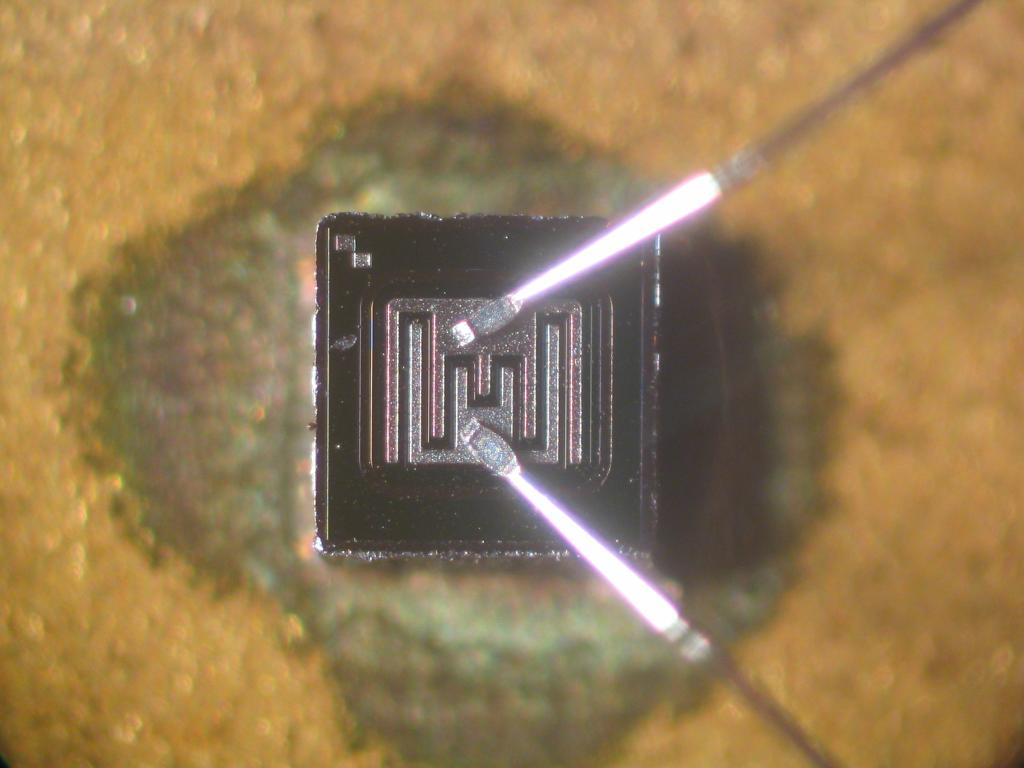
\includegraphics[scale=0.25]{pic/transistor}
\end{center}
}


\slide{Images on different pages}
{
\begin{center}
\includegraphics<1>[scale=0.125]{pic/transistor}
\pause
\includegraphics<2>[scale=0.25]{pic/transistor}
\end{center}
}


\slide{Image decorations}
{
\begin{itemize}
\item Lorem ipsum dolor sit amet,
\item consectetur adipisicing elit,
\item sed do eiusmod tempor incididunt
\item ut labore et dolore magna aliqua.
\item Ut enim ad minim veniam, quis
\item nostrud exercitation ullamco laboris
\item nisi ut aliquip ex ea commodo consequat.
\item Duis aute irure dolor in reprehenderit
\item in voluptate velit esse cillum dolore
\item eu fugiat nulla pariatur.
\item Excepteur sint occaecat cupidatat
\item non proident, sunt in culpa qui officia
\item deserunt mollit anim id est laborum.
\end{itemize}
\insImg{0.8}{0.2}{0.05}{pic/transistor}
\pause

\insImgFr{2-}{0.8}{0.5}{0.08}{pic/transistor}
}


\slide{Images interleaved with text}
{
Lorem ipsum dolor sit amet, consectetur adipisicing elit, sed do eiusmod tempor incididunt ut labore et dolore magna aliqua.

\begin{center}
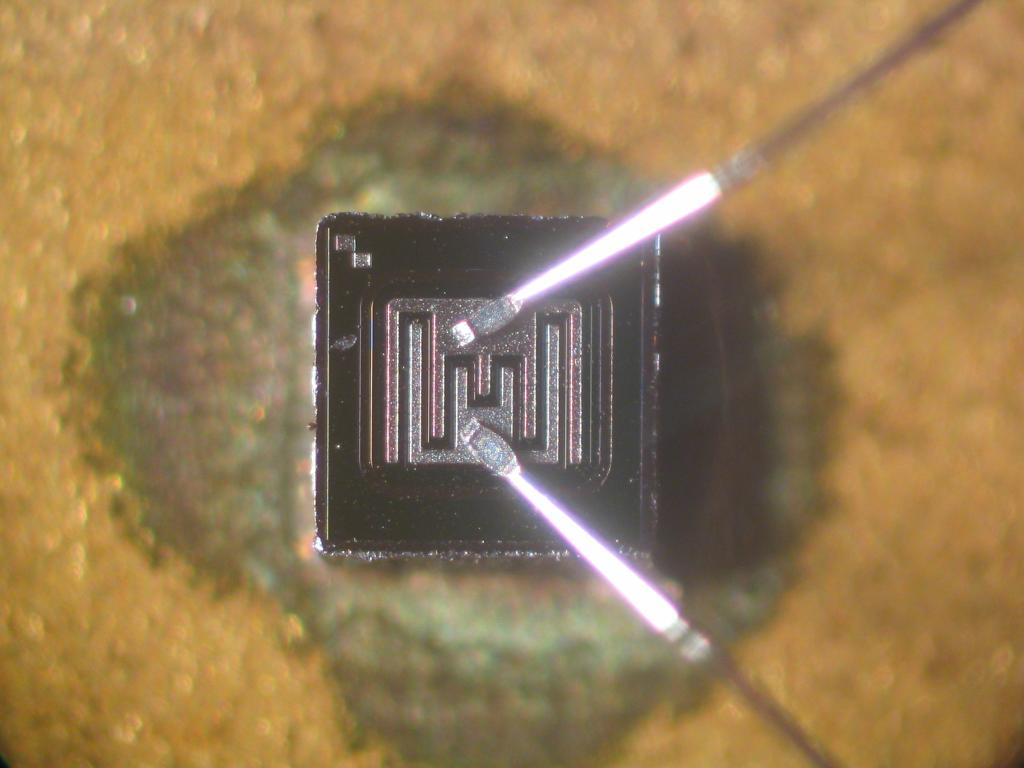
\includegraphics[scale=0.1]{pic/transistor}
\end{center}

Ut enim ad minim veniam, quis nostrud exercitation ullamco laboris nisi ut aliquip ex ea commodo consequat.
}


\slide{PNGs out of SVGs}
{
\begin{center}

\includegraphics[scale=0.5]{svg/biohazard}
\end{center}
}


\section{Graphviz}


\slide{Hello world}
{
\vspace{-1em}
\begin{center}
% NOTE: explain diagram in depth
\includegraphics[scale=0.8]{dot/sample}
\end{center}
}


\slide{Diagrams with seqdiag}
{
\vspace{-1em}
\begin{center}
\includegraphics[scale=0.66]{dot/connection}
\end{center}
}


\section{Gnuplot}


\slide{Function plot}
{
\begin{center}
\includegraphics[scale=0.7]{gnuplot/function}
\end{center}
}


\slide{Discrete plot}
{
\begin{center}
\includegraphics[scale=0.6]{gnuplot/points}
\end{center}
}


\section{Generating codes}


\slide{QR}
{
\begin{itemize}
\item QR codes are auto-generated
\item Put \emph{txt} file in \emph{qr/} directory
\item Insert text there
\item Image will be auto-generated
\end{itemize}

\begin{center}
% NOTE: explain diagram in depth
\includegraphics[scale=0.1]{qr/some_info}
\end{center}
}
